\pdfbookmark{Общая характеристика работы}{characteristic}             % Закладка pdf
\section*{Общая характеристика работы}

\newcommand{\actuality}{\pdfbookmark[1]{Актуальность}{actuality}\underline{\textbf{\actualityTXT}}}
\newcommand{\progress}{\pdfbookmark[1]{Разработанность темы}{progress}\underline{\textbf{\progressTXT}}}
\newcommand{\aim}{\pdfbookmark[1]{Цели}{aim}\underline{{\textbf\aimTXT}}}
\newcommand{\tasks}{\pdfbookmark[1]{Задачи}{tasks}\underline{\textbf{\tasksTXT}}}
\newcommand{\aimtasks}{\pdfbookmark[1]{Цели и задачи}{aimtasks}\aimtasksTXT}
\newcommand{\novelty}{\pdfbookmark[1]{Научная новизна}{novelty}\underline{\textbf{\noveltyTXT}}}
\newcommand{\influence}{\pdfbookmark[1]{Практическая значимость}{influence}\underline{\textbf{\influenceTXT}}}
\newcommand{\methods}{\pdfbookmark[1]{Методология и методы исследования}{methods}\underline{\textbf{\methodsTXT}}}
\newcommand{\defpositions}{\pdfbookmark[1]{Положения, выносимые на защиту}{defpositions}\underline{\textbf{\defpositionsTXT}}}
\newcommand{\reliability}{\pdfbookmark[1]{Достоверность}{reliability}\underline{\textbf{\reliabilityTXT}}}
\newcommand{\probation}{\pdfbookmark[1]{Апробация}{probation}\underline{\textbf{\probationTXT}}}
\newcommand{\contribution}{\pdfbookmark[1]{Личный вклад}{contribution}\underline{\textbf{\contributionTXT}}}
\newcommand{\publications}{\pdfbookmark[1]{Публикации}{publications}\underline{\textbf{\publicationsTXT}}}

{\actuality} Магнитоэлектрические эффекты обусловлены наличием в термодинамическом потенциале членов, линейных как по электрическому, так и по магнитному полю \autocite{Landau}. Данные эффекты наблюдаются в магнитоэлектриках и мультиферроиках в случае, когда одновременно нарушается симметрия относительно обращения знака времени (следствие магнитного упорядочения) и симметрия относительно пространственной инверсии (особенности кристаллической структуры) - магнитными свойствами этих материалов можно управлять прикладывая внешнее электрическое поле и наоборот. Так, авторы работы \autocite{Saito2008ape} наблюдали в антиферромагнетике \cbo\ вращение намагниченности, индуцированное электрическим полем. Позднее другая группа смогла управлять электрической поляризацией \ncbo\ с помощью внешнего магнитного поля \autocite{Khanh2013}. Кроме указанных \emph{статических} магнитоэлектрических эффектов наблюдаются также \emph{динамические} - обусловленные взаимодействием с периодическими электромагнитными полями. В частности, к таковым относятся явление невзаимности (nonreciprocity) в спектрах поглощения \autocite{Toyoda2015} и явление пространственной асимметрии люминесценции (directional asymmetry of luminescence) \autocite{Toyoda2016}.  

Интерес к этим эффектам в последние десятилетия существенно возрос, в связи с реальными перспективами практических применений. На основе магнитоэлектрических материалов можно создавать магнитные запоминающие устройства с оптическим считыванием информации о доменной структуре, управляемые магнитным полем оптические диоды и пр. Выяснение микроскопической природы (механизмов) этих эффектов важно для фундаментальных научных знаний.

\begin{figure}[ht]
	\centerfloat{
		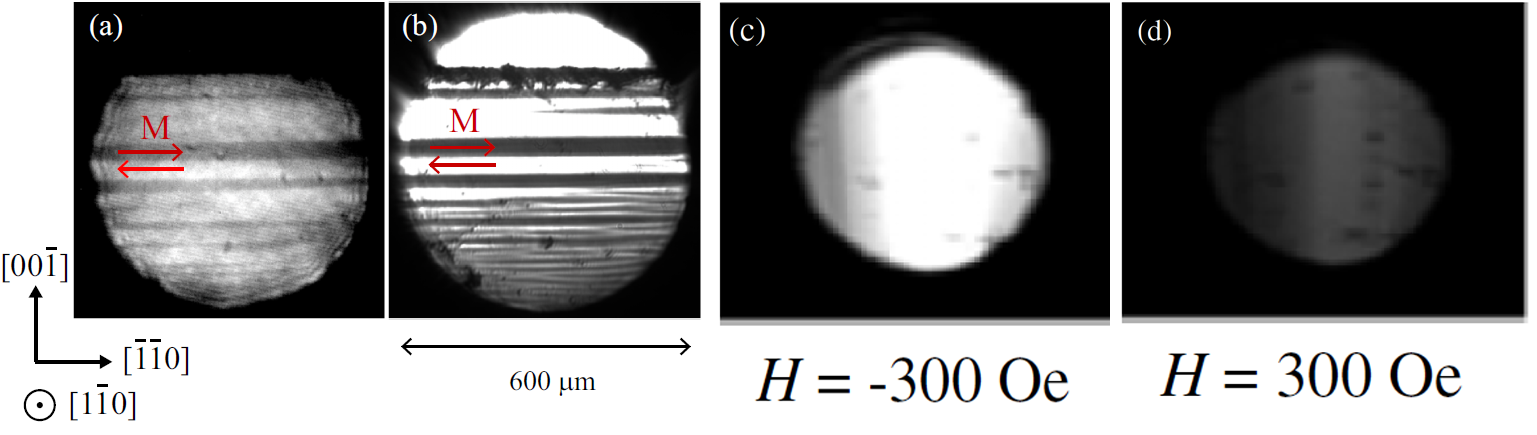
\includegraphics[scale=0.4]{applications}
	}
	\caption{(a), (b) Фотографии магнитных доменов из \autocite{Toyoda2016}, полученные с помощью фотолюминесценции. (c), (d) Фотографии света, прошедшего через пластинку \cbo\, к которой приложили внешнее магнитное поле в -300 и 300~Э~\autocite{Saito2008jpsj}. (a, b) и (c, d) сделаны при одной и той же яркости и контрасте.}\label{fig:applications}
\end{figure}

Можно выделить два подхода в развитии теории магнитоэлектрических эффектов: феноменологический и микроскопический. Феноменологический подход сформулирован в работе Дзялошинского \autocite{Dzyaloshinskii1959}. Этот подход успешно использовался для анализа ряда материалов. Его применение описано во многих обзорах и оригинальных статьях \autocite{Zvezdin2008, Pyatakov2012, Popkov2016}. Микроскопический подход развит слабее и предполагает предварительный анализ энергетических схем уровней и взаимодействий магнитных ионов с обменными и электрическими полями. Как это подчеркивается в обзорах \autocite{Khomskii2009, Moskvin2009, Tokura2014, Shuai2015}, микроскопические механизмы магнитоэлектрической связи еще не вполне выяснены.

%(см. рисунок \cref{fig:applications})

{\aim} данной работы является разработка микроскопической теории статических и динамических магнитоэлектрических эффектов в диэлектрике \cbo\ на основе квантово-механического подхода.

Для~достижения поставленной цели необходимо было решить следующие {\tasks}:
\begin{enumerate}[beginpenalty=10000] % https://tex.stackexchange.com/a/476052/104425
	\item проанализировать и систематизировать имеющиеся на момент написания работы данные по экспериментальному наблюдению и теоретическому описанию магнитоэлектрических эффектов в \cbo;
	\item рассчитать уровни энергии и волновые функции иона меди 3d\(^9\) в кристалле \cbo
	\item оценить параметры взаимодействия электронов меди с электрическим и магнитным полем
	\item попытаться объяснить  имеющиеся экспериментальные данные на основе  единой микроскопической модели 
\end{enumerate}


{\novelty}
\begin{enumerate}[beginpenalty=10000] % https://tex.stackexchange.com/a/476052/104425
	\item Получен эффективный оператор, позволивший объяснить происхождение магнитоэлектрических эффектов в	Cu$_{(1-x)}$Ni$_x$B$_2$O$_4$. Установлено, что они, главным образом, обусловлены ионами \emph{никеля}, а не меди, как предполагалось ранее.  
	\item Построены теоретические диаграммы пространственной асимметрии фотолюминесценции в магнитных полях при различных направлениях  волнового вектора и векторов поляризации.
\end{enumerate}


{\probation}
Основные результаты работы докладывались~на трех конференциях:
\begin{enumerate}[beginpenalty=10000] % https://tex.stackexchange.com/a/476052/104425
	\item \textit{Нурмухаметов, А. Р.} Особенности экситонных зон Френкеля-Давыдова в антиферромагнетиках [Устный доклад] / А.~Р.~Нурмухаметов // Итоговая конференция Института Физики. --- 2021.
	\item \textit{Нурмухаметов, А. Р.} Магнитоэлектрическая связь в Cu\(_{1-x}\)Ni\(_{x}\)B\(_{2}\)O\(_{4}\) [Устный доклад] / А.~Р.~Нурмухаметов // Итоговая конференция Института Физики. --- 2022.
	\item \textit{Нурмухаметов, А. Р.} К теории необратимости в спектрах \cbo\ [Стендовый доклад] / А.~Р.~Нурмухаметов, М.~В.~Еремин // Нанофизика и наноэлектроника. Труды XXVI Международного симпозиума. --- 2022.
\end{enumerate}

Имеются две публикации в журналах:

\begin{enumerate}[beginpenalty=10000] % https://tex.stackexchange.com/a/476052/104425
	\item \textit{Еремин, М. В.} О магнитоэлектрической связи в \ncbo / М.~В.~Еремин, А.~Р.~Нурмухаметов // Письма в ЖЭТФ. --- 2021. --- Т.~114, \textnumero~1. --- С.~31-35. --- URL: \url{https://doi.org/10.31857/S1234567821130073}.
	\item \textit{Нурмухаметов, А. Р.} О магнитоэлектрической связи в \ncbo / А.~Р.~Нурмухаметов, М.~В.~Еремин // ЖЭТФ. --- 2022. --- Т.~162, \textnumero~3. --- С.~1-8. --- URL: \url{https://doi.org/10.31857/S0044451022090000}.
\end{enumerate}


 % Характеристика работы по структуре во введении и в автореферате не отличается (ГОСТ Р 7.0.11, пункты 5.3.1 и 9.2.1), потому её загружаем из одного и того же внешнего файла, предварительно задав форму выделения некоторым параметрам

%Диссертационная работа была выполнена при поддержке грантов \dots

%\underline{\textbf{Объем и структура работы.}} Диссертация состоит из~введения,
%четырех глав, заключения и~приложения. Полный объем диссертации
%\textbf{ХХХ}~страниц текста с~\textbf{ХХ}~рисунками и~5~таблицами. Список
%литературы содержит \textbf{ХХX}~наименование.

\pdfbookmark{Содержание работы}{description}                          % Закладка pdf
\section*{Содержание работы}
Во \underline{\textbf{введении}} обосновывается актуальность
исследований, проводимых в~рамках данной диссертационной работы,
приводится обзор научной литературы по~изучаемой проблеме,
формулируется цель, ставятся задачи работы, излагается научная новизна
и практическая значимость представляемой работы. В~последующих главах
сначала описывается общий принцип, позволяющий \dots, а~потом идёт
апробация на частных примерах: \dots  и~\dots.


\underline{\textbf{Первая глава}} посвящена \dots

картинку можно добавить так:
\begin{figure}[ht]
    \centerfloat{
        \hfill
        \subcaptionbox{\LaTeX}{%
            
\includegraphics[scale=0.27]{latex}}
        \hfill
        \subcaptionbox{Knuth}{%
            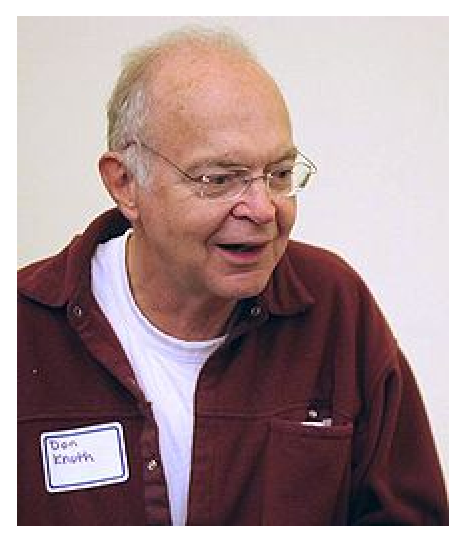
\includegraphics[width=0.25\linewidth]{knuth1}}
        \hfill
    }
    \caption{Подпись к картинке.}\label{fig:latex}
\end{figure}

Формулы в строку без номера добавляются так:
\[
    \lambda_{T_s} = K_x\frac{d{x}}{d{T_s}}, \qquad
    \lambda_{q_s} = K_x\frac{d{x}}{d{q_s}},
\]

\underline{\textbf{Вторая глава}} посвящена исследованию

\underline{\textbf{Третья глава}} посвящена исследованию

Можно сослаться на свои работы в автореферате. Для этого в файле
\verb!Synopsis/setup.tex! необходимо присвоить положительное значение
счётчику \verb!\setcounter{usefootcite}{1}!. В таком случае ссылки на
работы других авторов будут подстрочными.
Изложенные в третьей главе результаты опубликованы в~\cite{vakbib1, vakbib2}.
Использование подстрочных ссылок внутри таблиц может вызывать проблемы.

В \underline{\textbf{четвертой главе}} приведено описание

\FloatBarrier
\pdfbookmark{Заключение}{conclusion}                                  % Закладка pdf
В \underline{\textbf{заключении}} приведены основные результаты работы, которые заключаются в следующем:
%% Согласно ГОСТ Р 7.0.11-2011:
%% 5.3.3 В заключении диссертации излагают итоги выполненного исследования, рекомендации, перспективы дальнейшей разработки темы.
%% 9.2.3 В заключении автореферата диссертации излагают итоги данного исследования, рекомендации и перспективы дальнейшей разработки темы.
\begin{enumerate}
  \item На основе анализа \ldots
  \item Численные исследования показали, что \ldots
  \item Математическое моделирование показало \ldots
  \item Для выполнения поставленных задач был создан \ldots
\end{enumerate}


\pdfbookmark{Литература}{bibliography}                                % Закладка pdf
При использовании пакета \verb!biblatex! список публикаций автора по теме
диссертации формируется в разделе <<\publications>>\ файла
\verb!common/characteristic.tex!  при помощи команды \verb!\nocite!

\ifdefmacro{\microtypesetup}{\microtypesetup{protrusion=false}}{} % не рекомендуется применять пакет микротипографики к автоматически генерируемому списку литературы
\urlstyle{rm}                               % ссылки URL обычным шрифтом
\ifnumequal{\value{bibliosel}}{0}{% Встроенная реализация с загрузкой файла через движок bibtex8
    \renewcommand{\bibname}{\large \bibtitleauthor}
    \nocite{*}
    \insertbiblioauthor           % Подключаем Bib-базы
    %\insertbiblioexternal   % !!! bibtex не умеет работать с несколькими библиографиями !!!
}{% Реализация пакетом biblatex через движок biber
    % Цитирования.
    %  * Порядок перечисления определяет порядок в библиографии (только внутри подраздела, если `\insertbiblioauthorgrouped`).
    %  * Если не соблюдать порядок "как для \printbibliography", нумерация в `\insertbiblioauthor` будет кривой.
    %  * Если цитировать каждый источник отдельной командой --- найти некоторые ошибки будет проще.
    %
    %% authorvak
    \nocite{vakbib1}%
    \nocite{vakbib2}%
    %
    %% authorwos
    \nocite{wosbib1}%
    %
    %% authorscopus
    \nocite{scbib1}%
    %
    %% authorpathent
    \nocite{patbib1}%
    %
    %% authorprogram
    \nocite{progbib1}%
    %
    %% authorconf
    \nocite{confbib1}%
    \nocite{confbib2}%
    %
    %% authorother
    \nocite{bib1}%
    \nocite{bib2}%

    \ifnumgreater{\value{usefootcite}}{0}{
        \begin{refcontext}[labelprefix={}]
            \ifnum \value{bibgrouped}>0
                \insertbiblioauthorgrouped    % Вывод всех работ автора, сгруппированных по источникам
            \else
                \insertbiblioauthor      % Вывод всех работ автора
            \fi
        \end{refcontext}
    }{
        \ifnum \totvalue{citeexternal}>0
            \begin{refcontext}[labelprefix=A]
                \ifnum \value{bibgrouped}>0
                    \insertbiblioauthorgrouped    % Вывод всех работ автора, сгруппированных по источникам
                \else
                    \insertbiblioauthor      % Вывод всех работ автора
                \fi
            \end{refcontext}
        \else
            \ifnum \value{bibgrouped}>0
                \insertbiblioauthorgrouped    % Вывод всех работ автора, сгруппированных по источникам
            \else
                \insertbiblioauthor      % Вывод всех работ автора
            \fi
        \fi
        %  \insertbiblioauthorimportant  % Вывод наиболее значимых работ автора (определяется в файле characteristic во второй section)
        \begin{refcontext}[labelprefix={}]
            \insertbiblioexternal            % Вывод списка литературы, на которую ссылались в тексте автореферата
        \end{refcontext}
        % Невидимый библиографический список для подсчёта количества внешних публикаций
        % Используется, чтобы убрать приставку "А" у работ автора, если в автореферате нет
        % цитирований внешних источников.
        \printbibliography[heading=nobibheading, section=0, env=countexternal, keyword=biblioexternal, resetnumbers=true]%
    }
}
\ifdefmacro{\microtypesetup}{\microtypesetup{protrusion=true}}{}
\urlstyle{tt}                               % возвращаем установки шрифта ссылок URL
